\documentclass{article}
\usepackage{graphicx} % Required for inserting images
\usepackage{hyperref}

\title{Documentazione progetto Intelligenza Artificiale}
\author{Leonardo Vorabbi, Carlotta Nunziati}
\date{Marzo 2025}

\begin{document}

\maketitle

\section{Introduzione}
\paragraph{Problema} I CAPTCHA di nuova generazione sono più sicuri dei CAPTCHA tradizionali?

\paragraph{Tesi} È possibile implementare dei bot in grado di automatizzare la loro risoluzione.

\subsection{Rilevanza del problema} I CAPTCHA (Completely Automated Public Turing test to tell Computers and Humans Apart) sono sistemi di sicurezza ideati per distinguere tra utenti umani e bot. I CAPTCHA vengono utilizzati per impedire ai Web crawler automatizzati, noti anche come bot, di inviare commenti, moduli o spam sui siti Web e per difendersi da minacce online in senso lato (come attacchi DDoS, malvertising o attacchi ransomware). I CAPTCHA si sono evoluti per tenere il passo con le tecnologie sempre più sofisticate dei bot: se inizialmente questi test si basavano su immagini contenenti lettere, numeri o oggetti da riconoscere - compiti che richiedevano necessariamente l'intervento umano per la loro risoluzione - con l'evoluzione dell'intelligenza artificiale, molti CAPTCHA tradizionali sono diventati obsoleti e vulnerabili agli attacchi automatizzati, rendendo indispensabile lo sviluppo di soluzioni più avanzate. 

Il problema dei CAPTCHA interessa diversi gruppi di utenti, ad esempio sviluppatori di sicurezza informatica, che cercano nuovi metodi per proteggere le piattaforme online dagli attacchi automatizzati, oppure ricercatori di intelligenza artificiale e apprendimento automatico, che studiano sia i meccanismi di attacco ai CAPTCHA che le contromisure più efficaci. Ancora, il problema riguarda aziende e fornitori di servizi online, che necessitano di metodi affidabili per garantire l'autenticità degli utenti senza compromettere l'usabilità. Infine, il problema risulta rilevante anche per gli utenti finali, che interagiscono quotidianamente con i CAPTCHA e potrebbero beneficiare di metodi più intuitivi e meno frustranti.

\subsection{Soluzione proposta} La soluzione proposta permette di dimostrare la vulnerabilità dei CAPTCHA moderni, evidenziando le loro debolezze e incentivando lo sviluppo di soluzioni più sicure. Analizzando le tecniche per automatizzarne la risoluzione, è infatti possibile progettare metodi di protezione più avanzati, rendendo questi sistemi più resistenti agli attacchi. In questo modo, il lavoro non si limita a dimostrare le vulnerabilità dei sistemi esistenti, ma stimola anche l’innovazione nella protezione delle piattaforme online. Il progetto inoltre si propone di offrire un contributo rilevante all’esperienza utente: dimostrando che questi test non sono realmente efficaci nel bloccare i bot, ripensare i metodi di autenticazione si apre come l’unica via possibile per sviluppare soluzioni alternative più intuitive e meno intrusive. 

\section{Soluzione proposta}

\subsection{Approccio alla soluzione}
Abbiamo testato manualmente i CAPTCHA forniti da GeeTest
(\url{https://www.geetest.com/en/adaptive-captcha-demo}). 
Selezionando Slide CAPTCHA e Click to verify compare una schermata simile a quella di seguito:

\begin{figure}[h!]
    \centering
    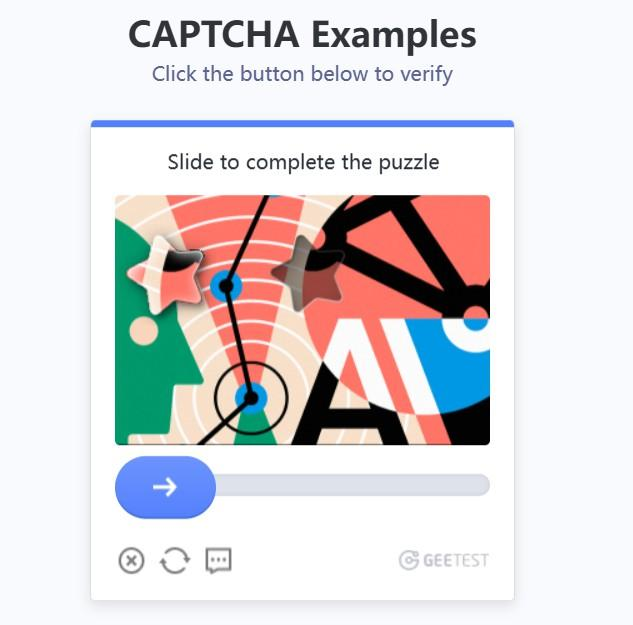
\includegraphics[width=0.5\linewidth]{captcha.jpeg}
    \caption{Esempio di CAPTCHA puzzle}
    \label{captcha}
\end{figure}

L’obiettivo è quello di trascinare con il cursore lo slider orizzontalmente fino a far coincidere il “pezzo di puzzle” con lo spazio che dovrebbe occupare: quando questi combaciano, lo slider deve essere rilasciato al fine di terminare la verifica. Viene considerato il movimento del cursore, che dovrebbe simulare quello umano, e la precisione nel posizionamento della figura.

Per dimostrare la nostra tesi, dobbiamo automatizzare la risoluzione del puzzle CAPTCHA.

\paragraph{Distribuzione dei compiti}
Per quanto riguarda la distribuzione dei compiti, Carlotta Nunziati si è occupata dell’utilizzo di Yolo per la risoluzione dei CAPTCHA attraverso Selenium mentre Leonardo Vorabbi sullo stesso approccio orientato al Reinforcement Learning e a quello basato su Template matching.

\subsection{Soluzioni individuate}

Abbiamo confrontato due diversi approcci per la risoluzione automatizzata dei CAPTCHA puzzle di GeeTest, analizzando l’efficacia e le differenze tra un metodo basato su intelligenza artificiale e uno più tradizionale senza AI.

\paragraph{Primo approccio} Il primo approccio sfrutta \textbf{YOLO} (You Only Look Once) per l’identificazione e il posizionamento del pezzo del puzzle. Il processo segue questi passi: navigazione alla pagina di GeeTest, raccolta delle immagini del puzzle (sia il pezzo da inserire che lo sfondo) tramite Selenium, analisi delle immagini con YOLO per identificare la posizione esatta del pezzo mancante, calcolo della distanza tra il pezzo da inserire e la bounding box rilevata nello sfondo, e infine interazione con la pagina web tramite Selenium per completare l’azione. L’uso di YOLO consente un rilevamento rapido e accurato del pezzo mancante, rendendo l’intero processo efficiente e scalabile.

\paragraph{Secondo approccio} Il secondo approccio utilizza invece il \textbf{template matching}, una tecnica classica del computational imaging basata sull’analisi delle immagini senza l’impiego di reti neurali. Il procedimento è simile al primo, ma con alcune differenze sostanziali: dopo la navigazione alla pagina e la raccolta delle immagini con Selenium, viene applicato un preprocessing delle immagini mediante edge detection con il metodo Canny. Successivamente, si esegue il template matching per individuare la posizione del pezzo mancante confrontando il pattern del pezzo con lo sfondo. Una volta rilevata la posizione, si calcola la distanza tra il pezzo da inserire e la bounding box nello sfondo, concludendo con l’interazione su pagina tramite Selenium per simulare il completamento del puzzle. 

\subsection{Problema nel problema}
Nelle soluzioni adottate, ci siamo scontrati con un ulteriore problema: la possibilità di simulare in modo realistico il movimento umano del mouse per evitare il rilevamento da parte dei sistemi anti-bot. Abbiamo esplorato due possibili soluzioni:

\paragraph{Prima soluzione} Movimento naturale attraverso un modello di Reinforcement Learning, in cui un agente viene addestrato a muovere il mouse verso un target, imitando i tempi di reazione e le piccole imprecisioni tipiche di un utente umano. 
\paragraph{Seconda soluzione } Utilizzo di Selenium con rumore casuale sulla traiettoria per aggiungere piccole deviazioni ai movimenti del mouse rispetto alla linea retta che collega il punto di partenza al punto di arrivo. In questo modo, si simulerebbe un comportamento più naturale, con variazioni casuali nel movimento, simili a come un essere umano sposterebbe il cursore.

\subsection{Valutazione}
Le prestazioni delle soluzioni adottate sono state valutate in base al tasso di successo nella risoluzione automatica dei CAPTCHA e alla velocità di esecuzione dell’operazione.

\section{Risultati}

\subsection{Istruzioni per l'esecuzione}

Il progetto è formato dalla seguente struttura:

\begin{figure}[h!]
    \centering
    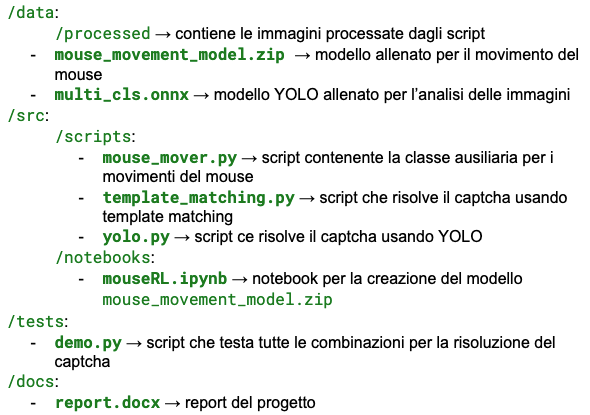
\includegraphics[width=1\linewidth]{struttura.png}
    \label{struttura}
\end{figure}

Per l’esecuzione degli script è necessario scaricare le dipendenze all’interno del file \texttt{requirements.txt} con il comando:
\begin{verbatim}
pip install -r requirements.txt
\end{verbatim}
Eseguendo il file \texttt{demo.py} si potranno automaticamente testare le varie soluzioni, mentre eseguendo \texttt{template\_matching.py} e \texttt{yolo.py} si potrà testare ogni soluzione singolarmente. Si noti che in quest'ultimo caso, negli import sarà necessario sostituire la riga:
\begin{verbatim}
from scripts.mouse_mover import MouseMover
\end{verbatim}
con la riga:
\begin{verbatim}
from mouse_mover import MouseMove
\end{verbatim}

Se si volesse allenare da zero il modello per lo spostamento del mouse, basterà importare il notebook \texttt{mouseRL.ipynb} all’interno di Google Colab (o simili) ed eseguirlo.

\subsection{Tecnologie e Versioni}

\begin{itemize}
    \item \textbf{Python} [v. 3.9.6]: linguaggio di programmazione ad alto livello.
    \item \textbf{Selenium} [v. 4.29.0]: libreria per l’automazione dei browser web, utilizzata per testare siti web e interagire con elementi delle pagine (come cliccare pulsanti o compilare form) tramite codice.
    \item \textbf{OpenAI Gym} [v. 0.25.2]: libreria open-source per sviluppare e testare algoritmi di reinforcement learning.
    \item \textbf{Stable Baselines3} [v. 2.5.0]: libreria di deep reinforcement learning basata su PyTorch, che fornisce implementazioni di algoritmi come PPO.
    \item \textbf{YOLO}: algoritmo di deep learning per il riconoscimento e la localizzazione di oggetti in immagini e video in tempo reale. Utilizza una rete neurale convoluzionale (CNN) per suddividere l’immagine in griglie e predire bounding box.
    \item \textbf{Google Colab}: piattaforma cloud di Google che permette di scrivere ed eseguire codice Python direttamente nel browser con supporto per GPU.
\end{itemize}

\subsection{Risultati della migliore configurazione}
Dopo aver testato diverse combinazioni di tecniche, la configurazione più efficace è risultata essere l’uso di YOLO per il riconoscimento del pezzo mancante e Selenium per l’interazione del bot con la pagina web. L’impiego di YOLO ha garantito un’elevata precisione nell’individuazione della posizione corretta del pezzo del puzzle da inserire. Il modello si è dimostrato robusto nel riconoscimento delle immagini, anche in presenza di leggere variazioni dovute a rumore, ombre o piccole modifiche nell’aspetto dei CAPTCHA. Il modello è stato in grado di identificare con grande accuratezza la bounding box del pezzo mancante, riducendo il margine di errore nel posizionamento del pezzo corretto. L’uso di Selenium per lo spostamento del mouse si è rivelato sufficiente, senza la necessità di utilizzare il modello di RL appositamente creato o aggiungere rumore casuale, in quanto il CAPTCHA non ha riconosciuto il movimento come sospetto. L’approccio si è rivelato semplice ed efficace: una volta ottenuta la posizione del pezzo mancante grazie a YOLO, il sistema ha calcolato la distanza esatta tra il pezzo da inserire e il punto corretto. Selenium ha quindi gestito il movimento del pezzo, effettuando il trascinamento e il rilascio in modo fluido e naturale. Questa configurazione ha permesso di completare i puzzle in tempi ridotti e con un’elevata precisione, senza essere rilevata dai sistemi anti-bot di GeeTest.

\subsection{Confronto tra le configurazioni}
Abbiamo valutato diverse configurazioni per l'automazione della risoluzione dei CAPTCHA puzzle di GeeTest:

\paragraph{YOLO + movimento base di Selenium (Migliore Configurazione)}
\begin{itemize}
    \item \textbf{Successo}: Alto
    \item \textbf{Velocità}: Alta
\end{itemize}

L’approccio basato su YOLO per il riconoscimento del pezzo mancante e il movimento del mouse base di Selenium per l’interazione con la pagina ha dimostrato il miglior compromesso tra accuratezza e velocità. YOLO ha permesso un rapido e preciso rilevamento della posizione corretta del pezzo, mentre Selenium ha gestito il trascinamento senza necessità di simulazioni avanzate del movimento umano. Questo ha portato a un’elevata percentuale di successo, con tempi di completamento inferiori rispetto agli altri metodi.

\paragraph{YOLO + Reinforcement Learning}
\begin{itemize}
    \item \textbf{Successo}: Alto, ma minore rispetto alla combinazione precedente
    \item \textbf{Velocità}: Bassa
\end{itemize}

L'uso di Reinforcement Learning per simulare un movimento umano realistico del mouse ha reso l’approccio accurato, riuscendo a evitare il rilevamento come bot. Tuttavia, la necessità di addestrare il modello e la complessità computazionale del calcolo delle traiettorie hanno reso questo metodo significativamente più lento. Seppur efficace, la maggiore latenza lo ha reso meno pratico per applicazioni in tempo reale.

\paragraph{Template Matching + movimento base di Selenium}
\begin{itemize}
    \item \textbf{Successo}: Medio
    \item \textbf{Velocità}: Alta
\end{itemize}

Il metodo basato su template matching per il riconoscimento del pezzo mancante e il movimento del mouse base di Selenium per l’interazione con la pagina ha mostrato risultati discreti, ma meno efficaci rispetto all'uso di YOLO. Il template matching è più sensibile a variazioni nelle immagini, come le distorsioni, riducendo l'affidabilità del riconoscimento. 

\section{Conclusioni}

\subsection{Discussione sui risultati}
Durante la fase di progettazione, ci aspettavamo che l'uso di YOLO per il riconoscimento visivo e di Selenium per l'interazione con la pagina web fosse un approccio efficace e relativamente veloce per risolvere i CAPTCHA puzzle. Tuttavia, c’erano diverse incognite da verificare:
\paragraph{Affidabilità del riconoscimento con YOLO}
Ci aspettavamo che YOLO fosse più robusto rispetto al template matching nel rilevare il pezzo mancante, ma non eravamo certi della sua precisione su immagini con variazioni di illuminazione o piccoli artefatti grafici.
\paragraph{Movimento del mouse di Selenium}
Una delle preoccupazioni era che il sito potesse rilevare l'automazione attraverso Selenium e bloccare l’accesso o generare CAPTCHA più difficili. Per questo è stato inizialmente sviluppato il modello RL per lo spostamento del mouse, in modo da far simulare a Selenium un movimento più umano. Tuttavia, il sito di GeeTest non ha sollevato questo problema, rendendo il modello addestrato essenzialmente inutile, essendo più lento e meno preciso. 
\paragraph{Reinforcement Learning per il movimento del mouse}
Si prevedeva che un modello di Reinforcement Learning potesse rendere il movimento più naturale, riducendo il rischio di rilevamento da parte di sistemi anti-bot. Tuttavia, non avevamo considerato che il suo utilizzo potesse introdurre una latenza significativa, rendendolo meno pratico rispetto alla semplice automazione con Selenium.

\subsection{Limiti e maturità tecnologica}
L'uso di Selenium, pur offrendo flessibilità nell'automazione, è soggetto a limitazioni imposte dai browser moderni e ai controlli sempre più stringenti adottati dai siti web per rilevare comportamenti automatizzati. 

\subsection{Lavori futuri}
I lavori futuri per un sistema di risoluzione di CAPTCHA possono concentrarsi sulla risoluzione di nuove tipologie di CAPTCHA, come "I'm not a robot" checkbox o i CAPTCHA basati su audio. Un altro possibile sviluppo riguarda il confronto tra i modelli pre-addestrati adottati e altri che non sono stati considerati in questo studio, al fine di comprendere se possano dimostrarsi maggiormente performanti. Visti inoltre i limiti di Selenium descritti nella sezione precedente, potrebbe valere la pena esplorare la possibilità di creare un modello più efficiente per l'automatizzazione del movimento del mouse seguendo una traiettoria "umana". Infine, un ulteriore passo avanti consisterebbe nell’applicare i modelli sviluppati a contesti reali, valutandone l’efficacia e l’adattabilità in scenari pratici.

\end{document}
